\begin{frame}{Steiner Forest Problem}
\begin{block}{Steiner Forest Problem}
 Dany jest graf nieskierowany $G = (V, E)$, funkcja kosztu $c: E \rightarrow Q^+$ oraz rodzina $S_1, \hdots, S_k$ podzbiorów rozłącznych $V$. Należy znaleźć podgraf $G$ o najmniejszym koszcie, w którym wierzchołki należące do tego samego zbioru są połączone.
\end{block}
\end{frame}

\begin{frame}{Steiner Forest Problem}
\begin{figure}[ht]
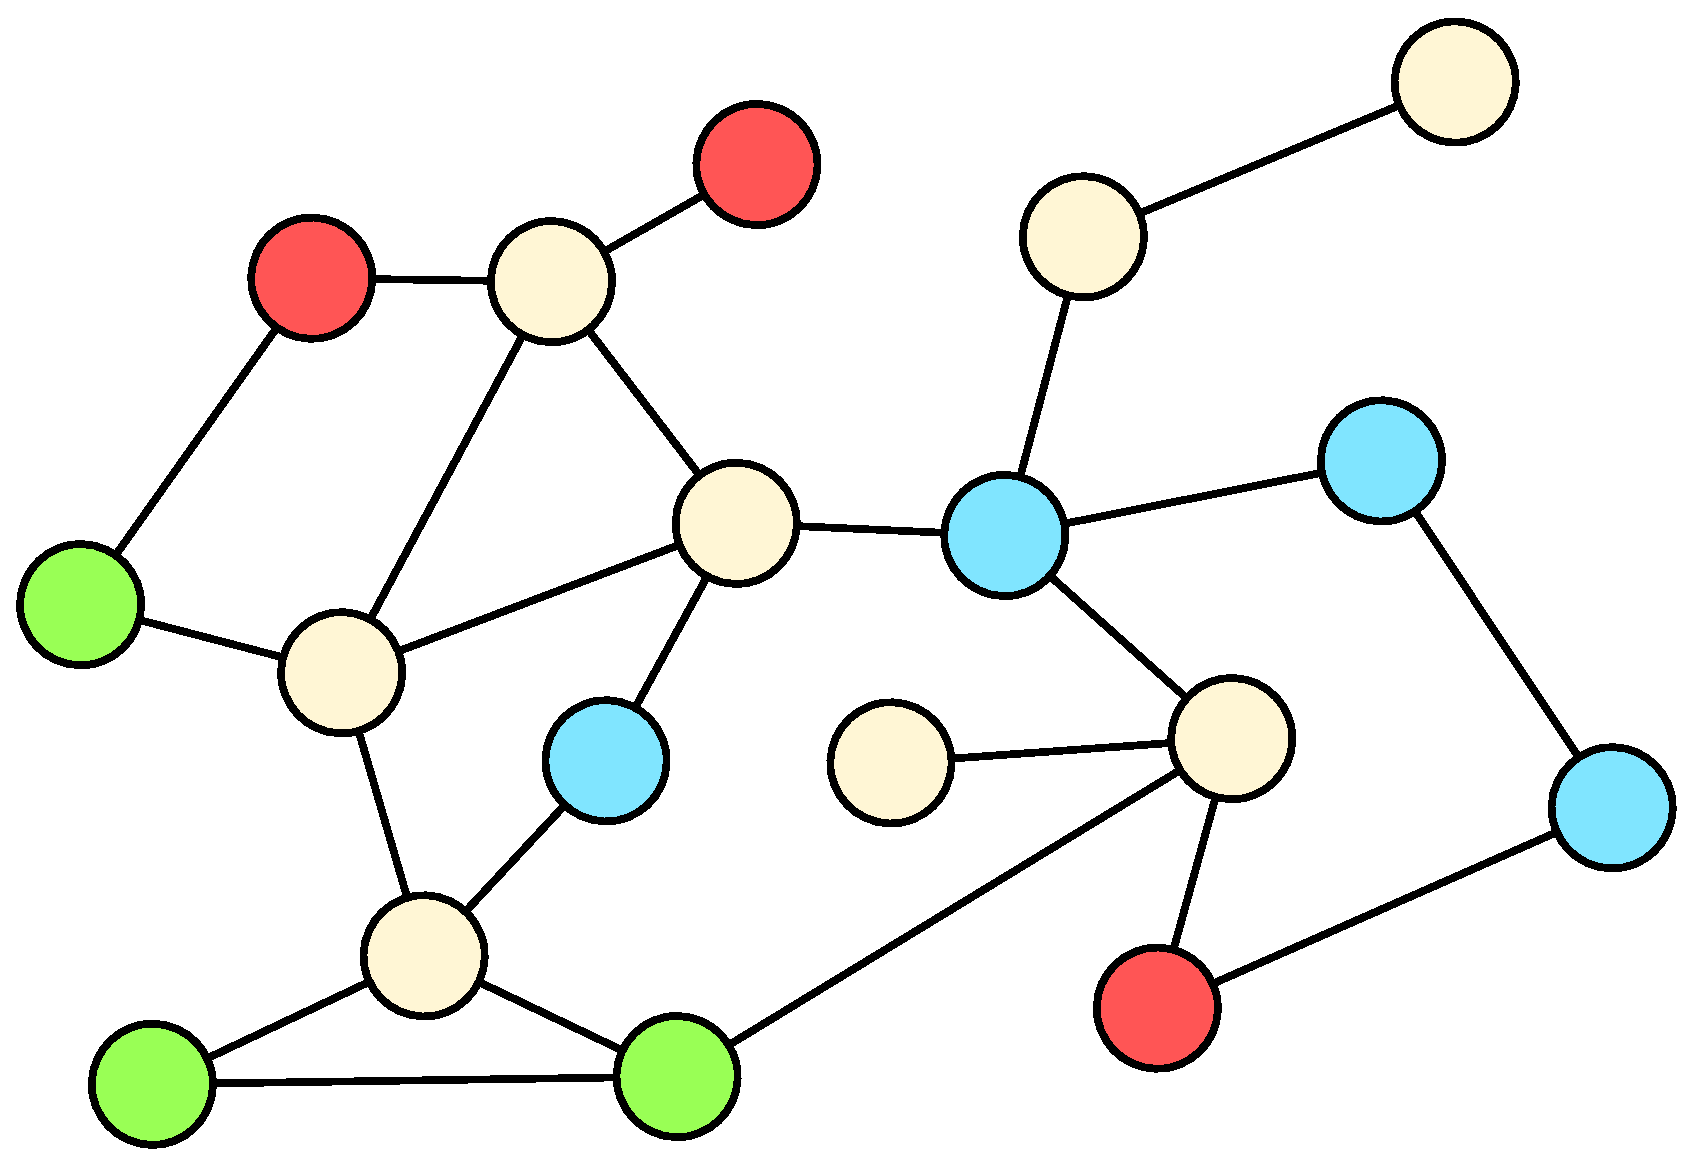
\includegraphics[scale=0.32]{sf_example.eps}
\end{figure}
\end{frame}

\begin{frame}{Steiner Forest Problem}
\begin{figure}[ht]
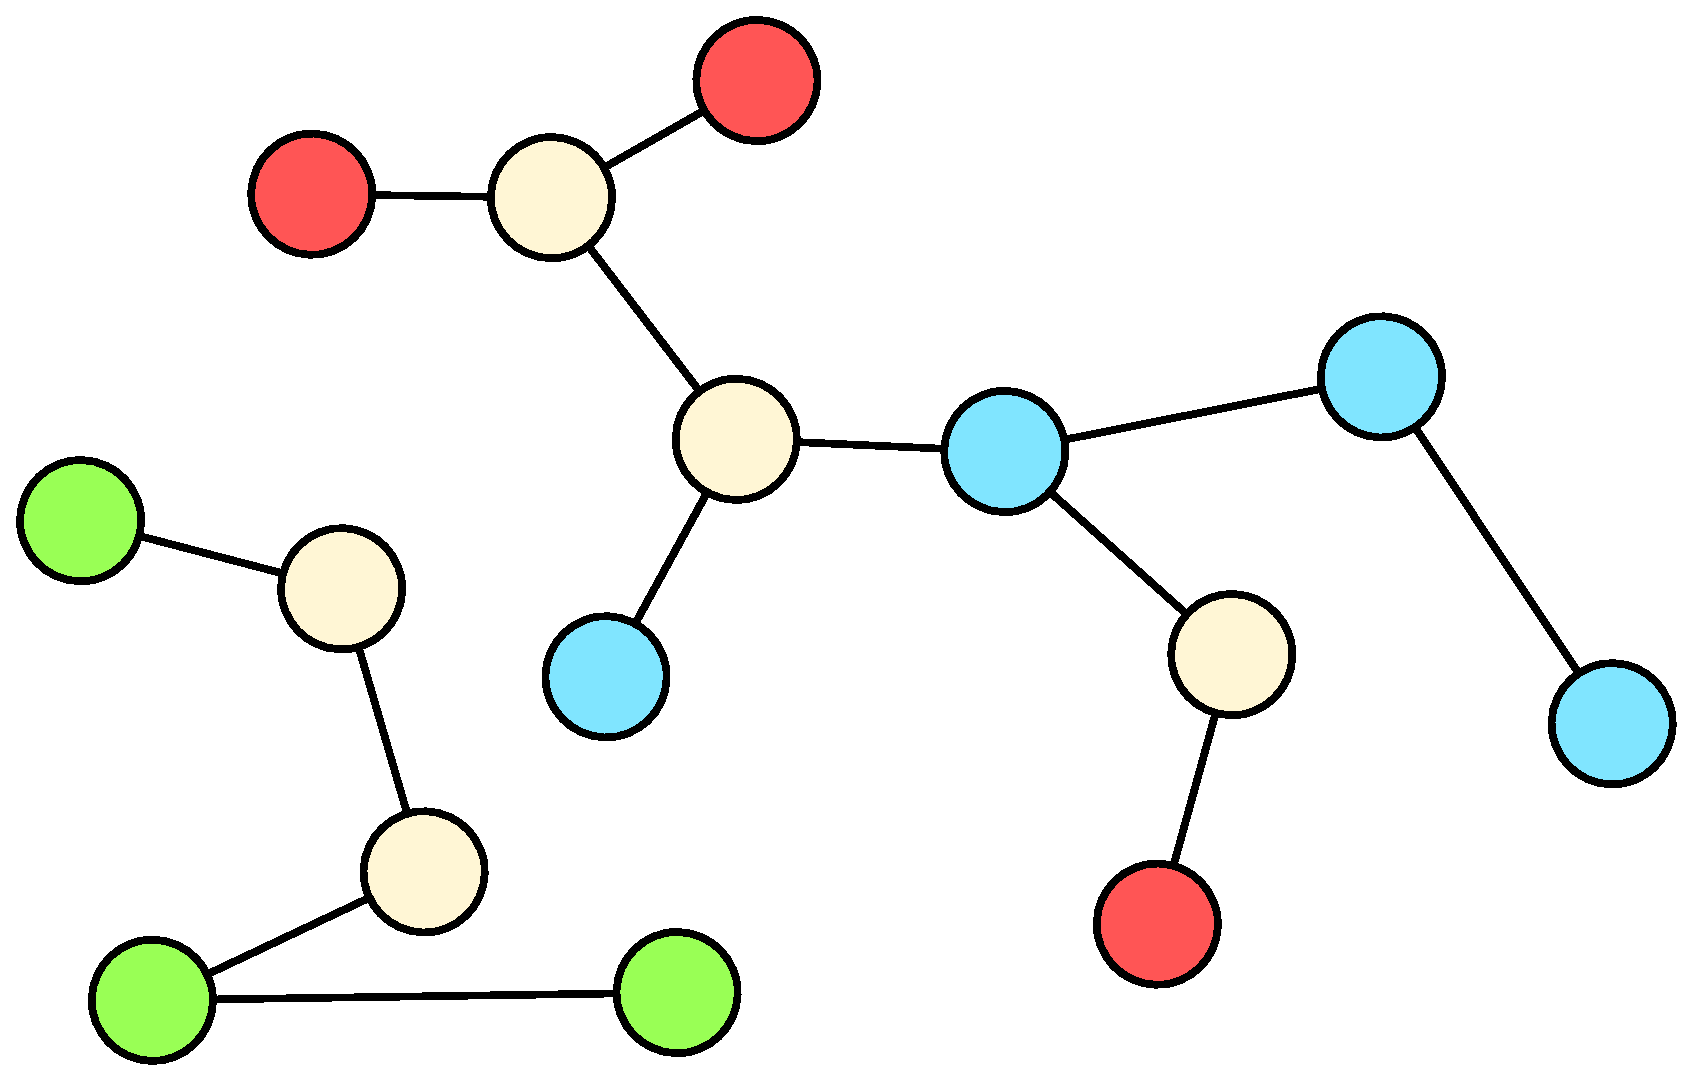
\includegraphics[scale=0.32]{sf_example2.eps}
\end{figure}
\end{frame}

\begin{frame}{Steiner Forest Problem}
\begin{figure}[ht]
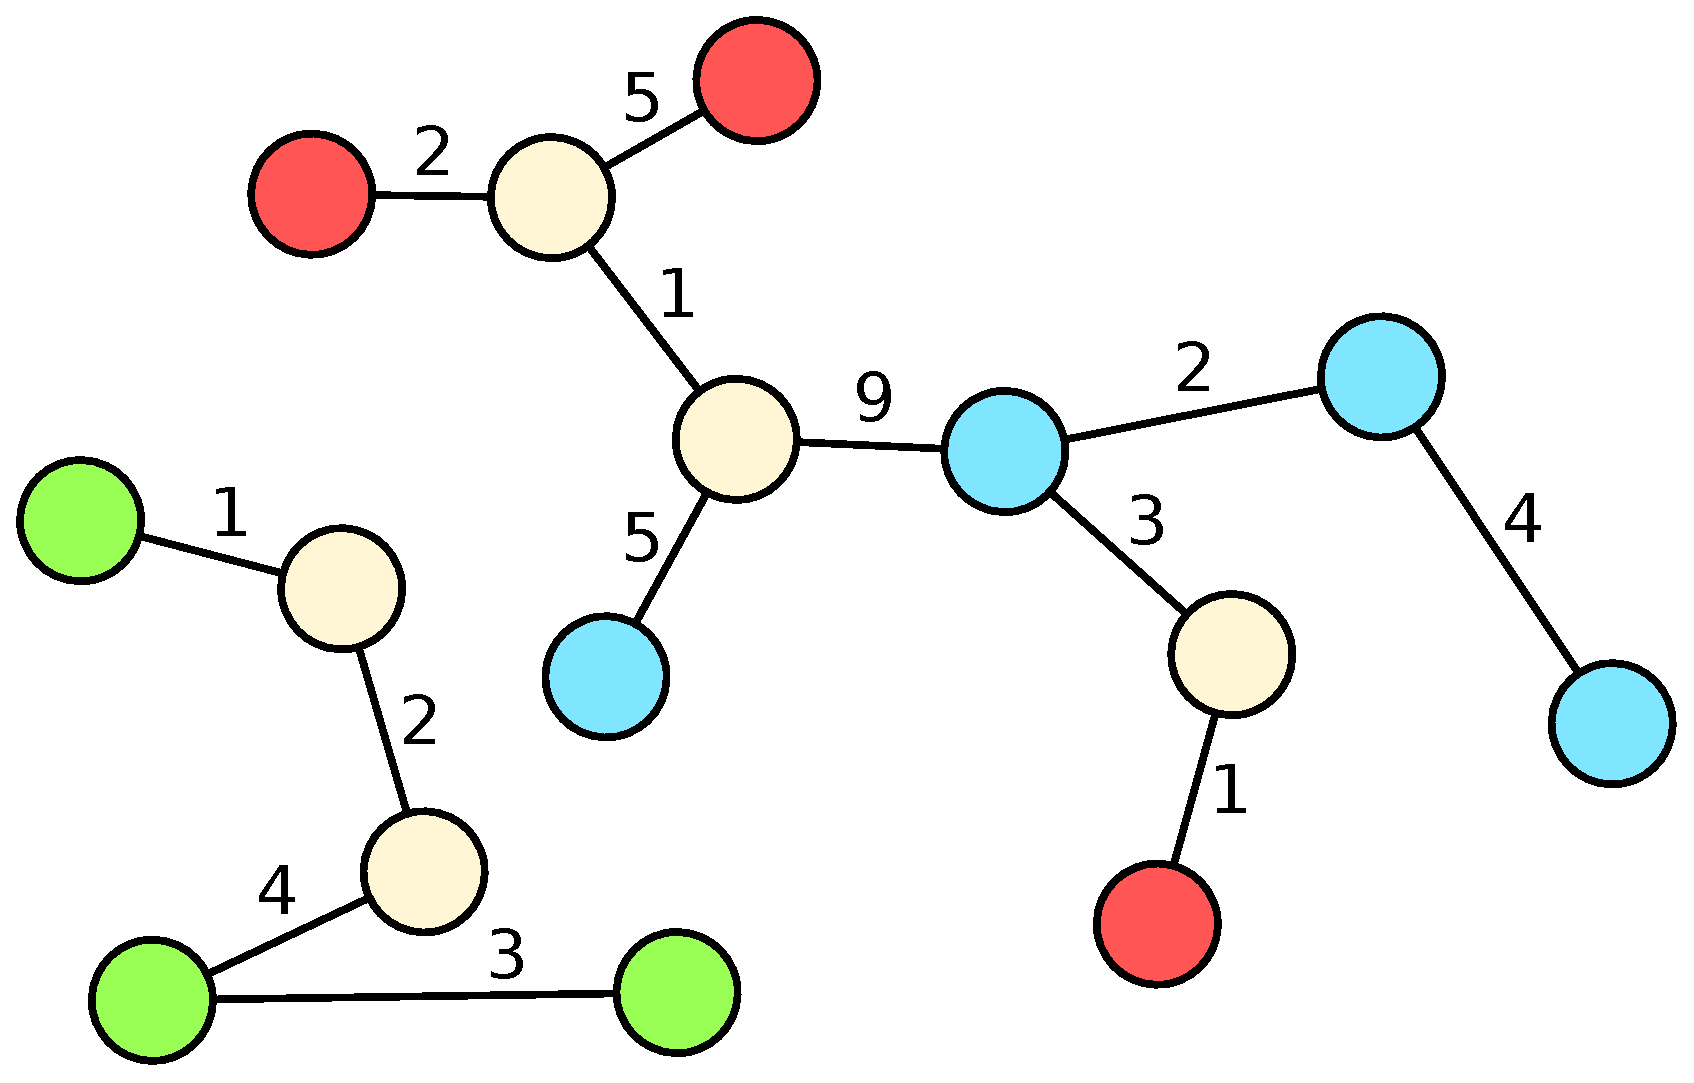
\includegraphics[scale=0.32]{sf_example3.eps}
\end{figure}
Sumując wagi krawędzi otrzymujemy koszt rozwiązania równy 42.
\end{frame}

\begin{frame}{Steiner Forest Problem}
\begin{block}{Algorytmy}
\begin{itemize}
\item 2-aproksymacja [Vazirani]
\item Dwa algorytmy oparte o metaheurystykę local search.
\end{itemize}
\end{block}
\end{frame}

\begin{frame}{Steiner Forest Problem}
\begin{block}{Obserwacje}
\begin{itemize}
\item Koszt rozwiązań znajdowanych przez algorytm 2-aproksymacyjny, nie większy niż 1.1 optimum.
\item Istotna przewaga jednego z algorytmów local search pod względem kosztu znalezionego rozwiązania nad drugim.
\item Lepszy z algorytmów local search znajduje rozwiązania tańsze niż algorytm 2-aproksymacyjny, w instancjach problemu gdzie graf ma do kilkuset wierzchołków.
\item Zmiana strategii z hill climbing na simulated annealing nie poprawia wyników.
\end{itemize}
\end{block}
\end{frame}

\begin{frame}{Steiner Forest Problem}
Dalsza lektura dla zainteresowanych:
\begin{thebibliography}{9}
\setbeamertemplate{bibliography item}[online]
\bibitem{paal} {\em http://students.mimuw.edu.pl/\textasciitilde ls306462/paal.pdf}
\setbeamertemplate{bibliography item}[book]
\bibitem{Vazirani} Vijay V. Vazirani, Algorytmy aproksymacyjne, WNT, Warszawa 2005
\end{thebibliography}
\end{frame}
